\begin{figure}[H]
\begin{center}
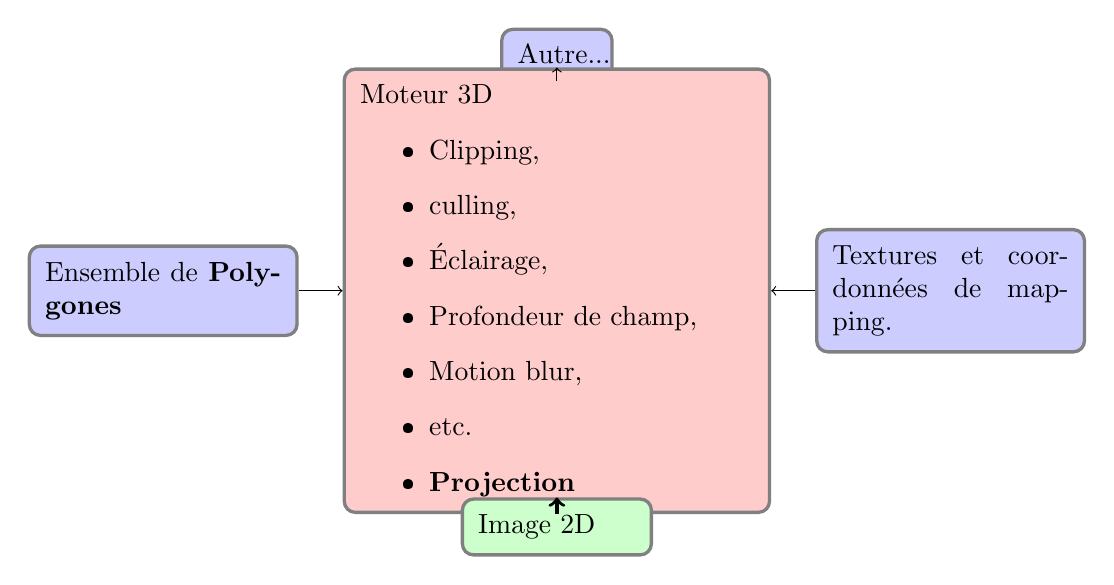
\begin{tikzpicture}
  [entree/.style={
    draw=black!50,
    fill=blue!20,
    rectangle,
    rounded corners,
    inner sep=.2cm,
    very thick}, systeme/.style={
    draw=black!50,
    fill=red!20,
    rectangle,
    rounded corners,
    inner sep=.2cm,
    very thick}, sortie/.style={
    draw=black!50,
    fill=green!20,
    rectangle,
    rounded corners,
    inner sep=.2cm,
    very thick}]

  \node [entree] at (-5,0) (polygone) {
  \begin{minipage}{3cm}
    Ensemble de \textbf{Polygones}
  \end{minipage}
  };

  \node [entree] at (5,0) (textures) {
  \begin{minipage}{3cm}
    Textures et coordonnées de mapping.
  \end{minipage}
  };

  \node [entree] at (0,3) (other) {
  \begin{minipage}{1cm}
    Autre...
  \end{minipage}
  };

  \node [systeme] (engine) {
  \begin{minipage}{5cm}
    Moteur 3D 
    \begin{itemize}
      \item Clipping,
      \item culling,
      \item Éclairage,
      \item Profondeur de champ,
      \item Motion blur,
      \item etc.
      \item \textbf{Projection}
    \end{itemize}
  \end{minipage}
  };

  \node [sortie] at (0,-3) (image) {
  \begin{minipage}{2cm}
    Image 2D
  \end{minipage}
  };

  \draw [->] (polygone) -- (engine);
  \draw [->] (textures) -- (engine);
  \draw [->] (other) -- (engine);
  \draw [very thick, ->] (engine) -- (image);
\end{tikzpicture}
\caption{Représentation grossière du pipeline de rendu via la
rasterisation\label{rasterisationPipeline}}
\end{center}

\end{figure}
